\documentclass{article}
\usepackage[utf8]{inputenc}
\usepackage{graphicx} 
\usepackage{fancyhdr}
\usepackage{ragged2e}
\usepackage{multirow}
\usepackage[hidelinks]{hyperref}
\usepackage[table,xcdraw]{xcolor}
\usepackage{ulem}
\usepackage{listings}
\usepackage[spanish]{babel} % Paquete para idioma español
\usepackage{xcolor} % Para usar colores

\usepackage{caption}

\usepackage{bbding}
\usepackage{pifont}
\usepackage{wasysym}
\usepackage{amssymb}


\definecolor{verdeCompletado}{RGB}{0, 128, 0} % Verde para tareas completadas
\definecolor{azulProgreso}{RGB}{30, 144, 255} % Azul para tareas en progreso
\definecolor{grisPendiente}{RGB}{169, 169, 169} % Gris para tareas pendientes



\usepackage{pgfgantt}
\usepackage{float}
\usepackage{pdflscape} % Paquete para la orientación horizontal
\usepackage{longtable} % Para tablas largas.
\usepackage{geometry} 
\usepackage{ragged2e}
\usepackage{translator}
\ganttset{calendar week text={\small{\startday/\startmonth}}}
\newcommand\textganttbar[5][]{%
    \ganttbar[#1,bar/.append style={alias=tmp}]{#2}{#4}{#5}
    \path 
    let
    \p1=(tmp.west),\p2=(tmp.east),
    \n1={\x2-\x1},\n2={width("#3")},
    \n3={ifthenelse(\n1>\n2,90,270)}
    in
    node [anchor=\n3,font=\footnotesize] at (tmp.north) {#3};
}

% Definir un color azul oscuro
\definecolor{azulOscuro}{RGB}{0, 0, 139} % Azul oscuro


% Adicionales
\addto\captionsspanish{\renewcommand{\contentsname}{Índice}} % Cambio de  Adicionales Contents a Indice
\pagestyle{fancy}
\fancyhf{}
\lhead{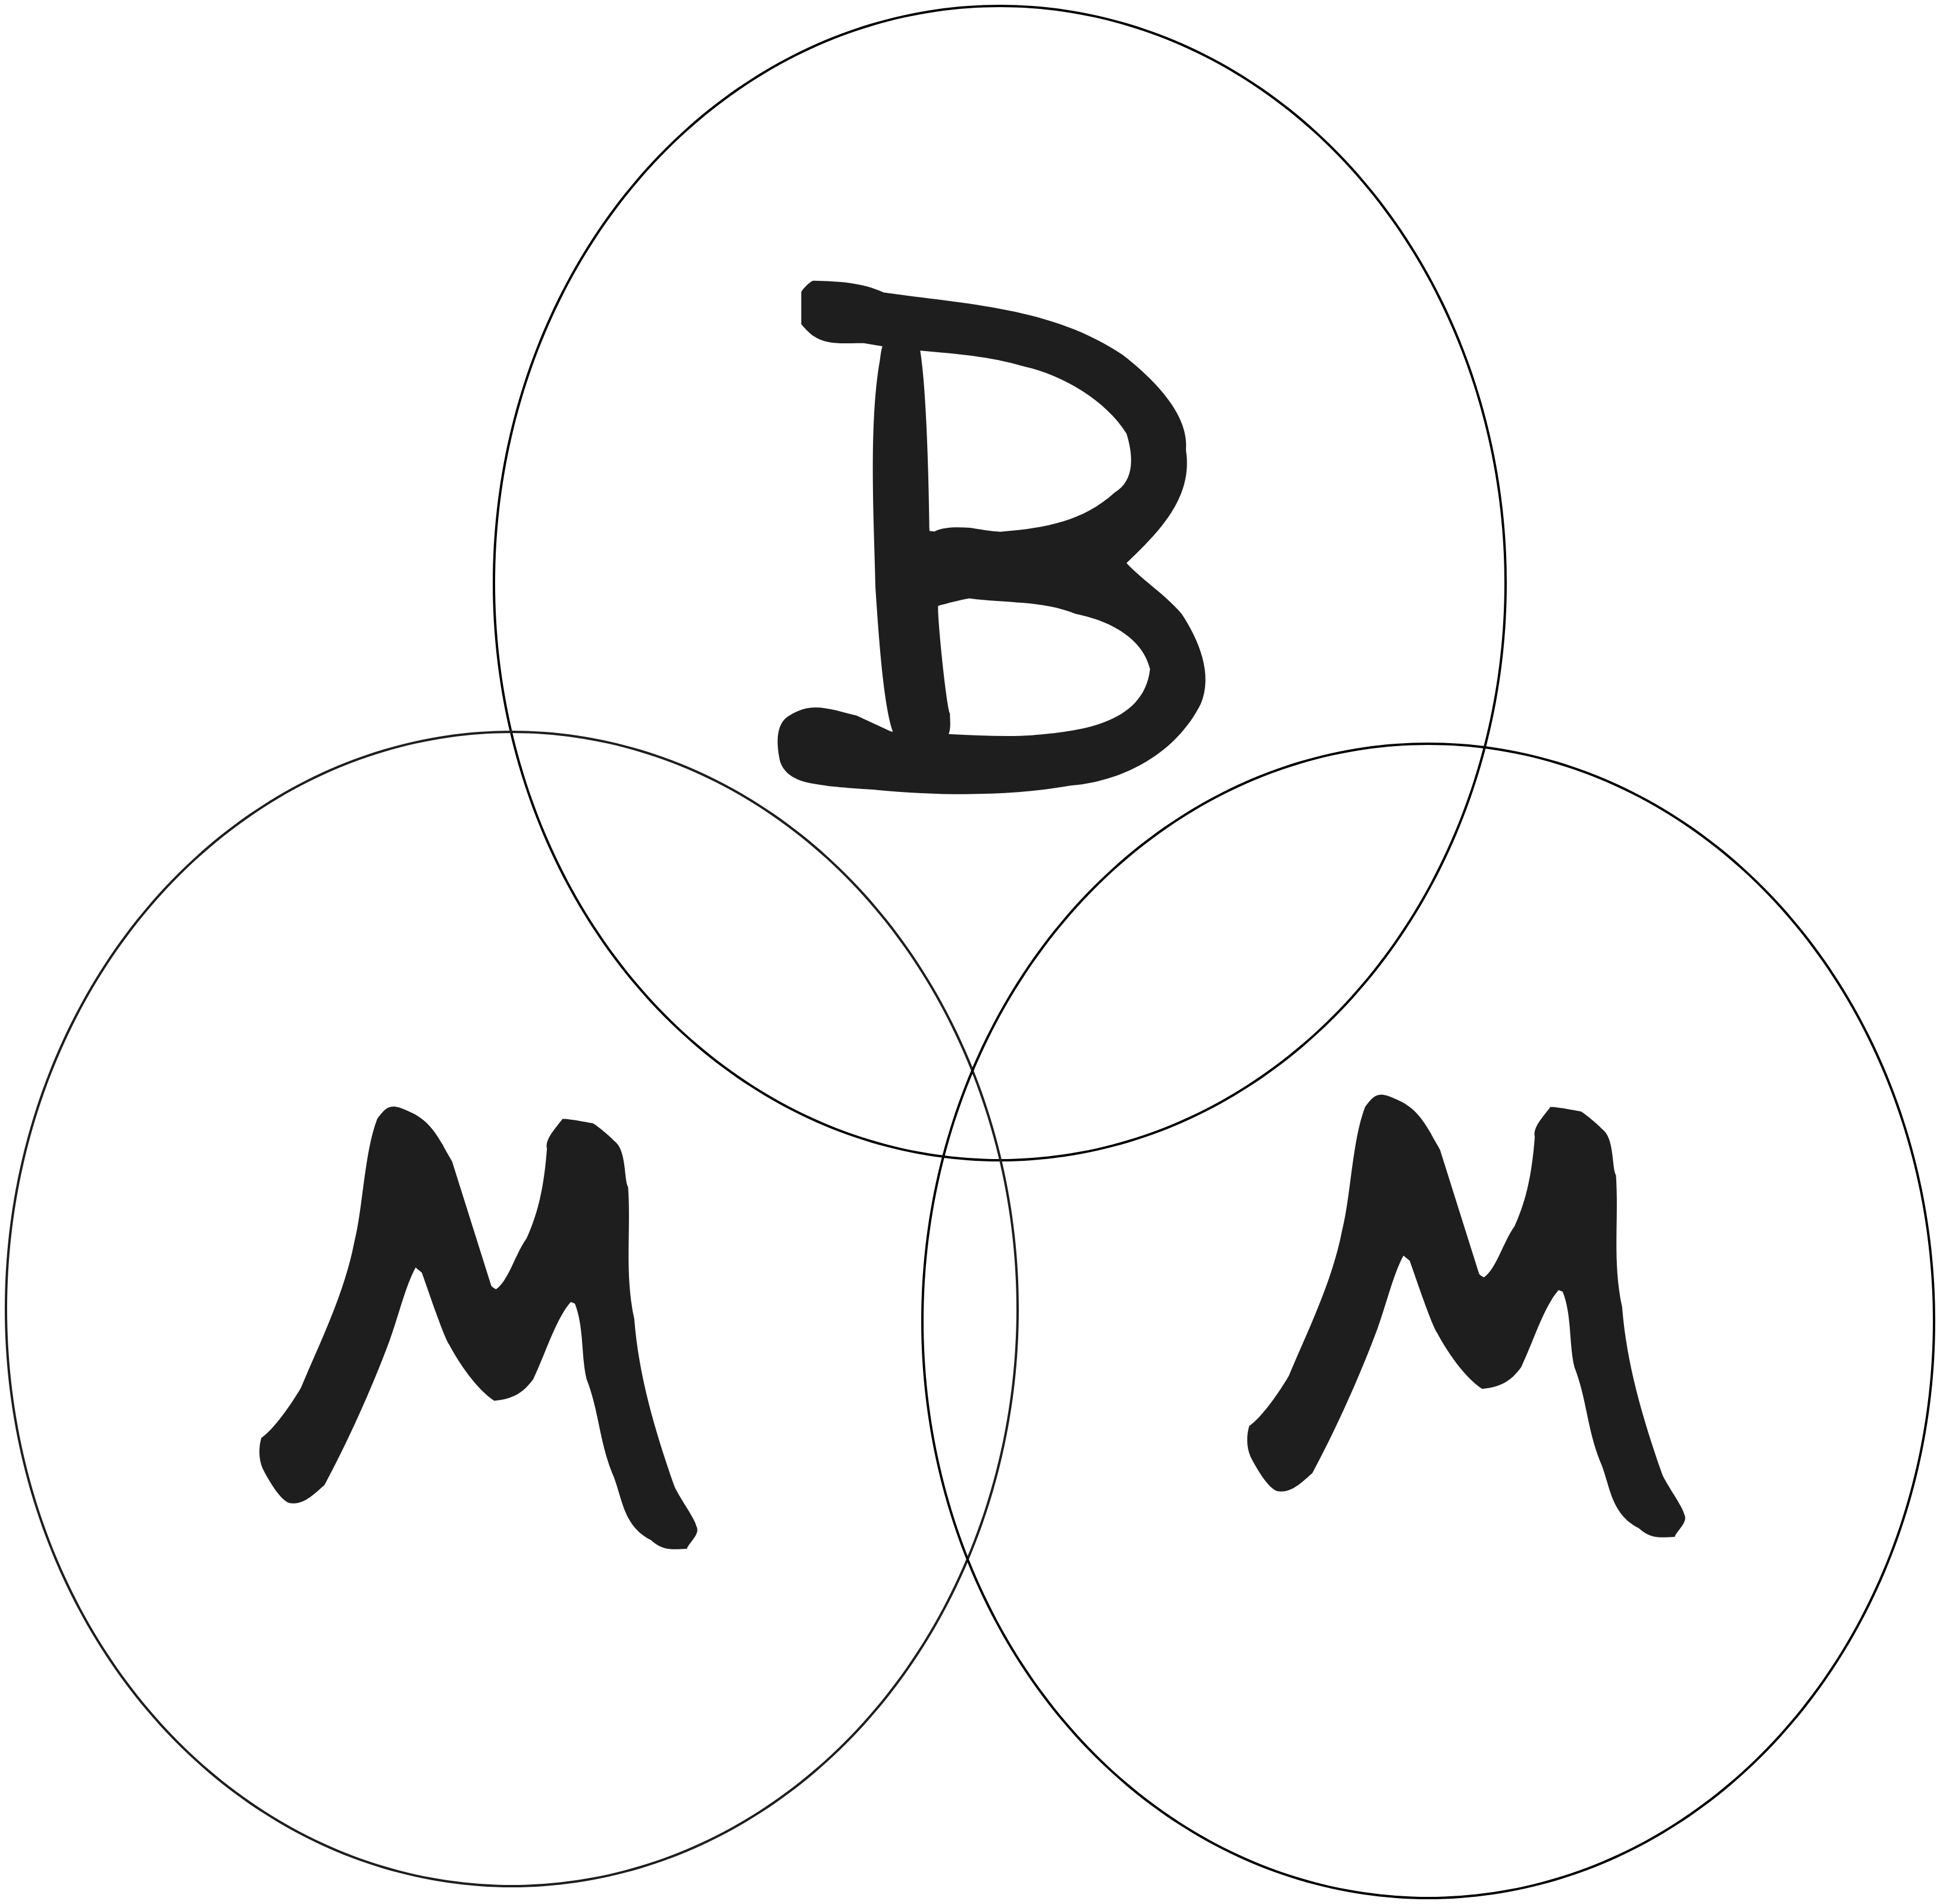
\includegraphics[width=1cm]{TFG/Logo.png}}

\renewcommand{\headrulewidth}{3pt}
   %Comienzo de Documento
    \begin{document}
            % Creacion de Portada----------------------------------------------------------
% Comienzo de Documento
    % Creación de Portada
    \begin{titlepage}
        \begin{center}
            {\scshape\large{Grado Superior}}\\
            {\scshape\large{Desarrollo de aplicaciones multiplataforma}} \\

            
            \vspace{2cm}
            {
\includegraphics[width=0.4\textwidth]{TFG/fotomain.png}} \par
            \vspace{2cm}
            {\scshape\large{ Aplicación para la Gestión de Tareas y Control \\ de Alimentos en el Hogar}\\
            \vspace{2cm}
            \textbf{TaskTracer}}} \\
            \vspace{2cm}
            {\Large Autor:} \\
            \vspace{1mm}
            {\Large Borja Merchán Mckenna} \\
            \vspace{1mm}
            {\Large 13/11/2024}
        \end{center}
    \end{titlepage}

 % ----------------------------------------------------------------
        %Comienzo de Toc
        
        \clearpage
        \tableofcontents

         \clearpage








    \section{Planificación completa del proyecto}
    \begin{table}[H]
    \centering
    \begin{tabular}{|l|l|}
        \hline
        \textbf{Clave} & \textbf{Funcionalidades} \\ \hline
         & Inicio de la Aplicación \\ \hline
        F1 & Nombre de la aplicación \\ \hline
        F2 & Logo de la aplicación \\ \hline
        F3 & Investigación de herramientas \\ \hline
         & Diseño de Aplicación \\ \hline
        F4 & Diagrama de Gantt \\ \hline
        F5 & Diagrama de flujo \\ \hline
        F6 & Diseñar en el front \\ \hline
         & Desarrollo \\ \hline
        F7 & Desarrollo de usuarios \\ \hline
        F8 & Desarrollo de grupo de hogar \\ \hline
        F9 & Desarrollo del to-do \\ \hline
        F10 & Desarrollo gestión de nevera \\ \hline
        F11 & Desarrollo de ajustes \\ \hline
         & Implementación en Firebase \\ \hline
        F12 & Implementación de firebase en usuarios \\ \hline
        F13 & Implementación de firebase en grupo de hogar \\ \hline
        F14 & Implementación de firebase en  el to-do \\ \hline
        F15 & Implementación de firebase en  gestión de nevera \\ \hline
        F16 & Implementación de firebase en  ajustes \\ \hline
         & Pruebas y Seguridad \\ \hline
        F17 & Implementación Mejoras  \\ \hline
        F18 & Mantenimiento y Actualización \\ \hline
         & Documentación \\ \hline
        F19 & Documentación en PDF \\ \hline
        F20 & Presentación en PowerPoint \\ \hline
    \end{tabular}
    \caption{Tabla de Funcionalidades}
    \label{tab:funcionalidades}
\end{table}


        \begin{figure}[H]
            \begin{ganttchart}[
            x unit=0.120cm, % distancia entre cada unidad horizontal (días).
            y unit chart=0.5cm, % altura de cada unidad vertical.
            y unit title=0.7cm, % altura de las filas de títulos.
            title height=1, % separación entre una fila de títulos y otra (1 = ninguna separación).
            hgrid, % dibujar las separaciones verticales.
            vgrid={*6{draw=none}, dotted}, % dibujar las separaciones verticales en intervalos semanales.
            bar/.append style={fill=white}, % barras de color blanco por defecto.
            group peaks width=3,
            group peaks tip position=0.5,
            group peaks height=.1, % distintos parámetros para el formato de los grupos.
            time slot format=isodate, % formato de las fechas.
            ] {2024-09-26}{2024-12-15} % inicio y final del eje temporal (año-mes-día).

            % Títulos:
            \gantttitle{Diagrama de Gantt: TaskTracer}{81} \\ % Título centrado y extendido
            \gantttitlecalendar{year, month=shortname} \\ 
            \gantttitlecalendar[title height=2, title label node/.append style={rotate=90}]{week} \\
            \gantttitle[title/.style={opacity=0}]{}{364} \\ 

            % Grupos y tareas:
            \ganttgroup{Inicio de la Aplicación}{2024-09-26}{2024-09-29} \\
            \ganttbar[bar/.append style={fill=blue!20}]{F1  \Large {\CheckedBox}}{2024-09-26}{2024-09-26} \\
            \ganttbar[bar/.append style={fill=blue!20}]{F2  \Large {\CheckedBox}}{2024-09-27}{2024-09-28} \\
            \ganttbar[bar/.append style={fill=blue!20}]{F3  \Large {\CheckedBox} }{2024-09-28}{2024-09-29} \\

            \ganttgroup{Diseño de Aplicación}{2024-09-30}{2024-10-16} \\
            \ganttbar[bar/.append style={fill=orange!50}]{F4 \Large {\CheckedBox}}{2024-09-30}{2024-10-04} \\
            \ganttbar[bar/.append style={fill=orange!50}]{F5 \Large {\CheckedBox}}{2024-10-05}{2024-10-08} \\
            \ganttbar[bar/.append style={fill=orange!50}]{F6 \Large {\CheckedBox}}{2024-10-12}{2024-10-16} \\

            \ganttgroup{Desarrollo}{2024-10-17}{2024-11-20} \\
            \ganttbar[bar/.append style={fill=green!50}]{F7 \Large {\CheckedBox}}{2024-10-17}{2024-10-22} \\
            \ganttbar[bar/.append style={fill=green!50}]{F8 \Large {\CheckedBox}}{2024-10-23}{2024-10-28} \\
            \ganttbar[bar/.append style={fill=green!50}]{F9  \Large {\CheckedBox}}{2024-10-29}{2024-11-03} \\
            \ganttbar[bar/.append style={fill=green!50}]{F10 \Large {\CheckedBox}}{2024-11-04}{2024-11-09} \\
            \ganttbar[bar/.append style={fill=green!50}]{F11 \Large {\CheckedBox}}{2024-11-10}{2024-11-15} \\ 

            
            \ganttgroup{Implementación en Firebase}{2024-10-17}{2024-11-20} \\

       \ganttbar[bar/.append style={fill=green!50}]{F12 \Large {\CheckedBox}}{2024-10-17}{2024-10-22} \\
            \ganttbar[bar/.append style={fill=green!50}]{F13 \Large {\CheckedBox}}{2024-10-23}{2024-10-28} \\
            \ganttbar[bar/.append style={fill=green!50}]{F14 \Large {\CheckedBox}}{2024-10-29}{2024-11-03} \\
            \ganttbar[bar/.append style={fill=green!50}]{F15 \Large {\CheckedBox}}{2024-11-04}{2024-11-09} \\
            \ganttbar[bar/.append style={fill=green!50}]{F16 \Large {\CheckedBox}}{2024-11-10}{2024-11-15} \\

            


             \ganttgroup{Pruebas y Seguridad}{2024-11-20}{2024-12-10} \\
         \ganttbar[bar/.append style={fill=green!50}]{F17 \Large {\XBox}}{2024-11-15}{2024-11-25} \\ 

            \ganttbar[bar/.append style={fill=red!50}]{F18 \Large {\XBox}}{2024-11-20}{2024-12-10} \\ 

            \ganttgroup{Documentación}{2024-11-20}{2024-12-15} \\
            \ganttbar[bar/.append style={fill=green!50}]{F19 \Large {\XBox}}{2024-11-20}{2024-12-15} \\ 
            \ganttbar[bar/.append style={fill=green!50}]{F20 \Large {\XBox}}{2024-12-10}{2024-12-15} \\ 


            % Relaciones de dependencia:

            \end{ganttchart}
            \caption{Diagrama de Gantt de TaskTracer}
            \label{fig:gantt}
        \end{figure}
        

\section{Ejecución Real frente a Ejecución Planificada}

El desarrollo de la aplicación se está llevando a cabo de forma adecuada, siguiendo en gran medida el plan definido inicialmente. Sin embargo, aunque gran parte de la funcionalidad ya está implementada, todavía quedan algunos aspectos por mejorar y finalizar. Entre las tareas pendientes se encuentran:

\begin{itemize}
    \item Optimizar el flujo de usuario para que, si ya pertenece a un grupo de hogar, no se muestre la pantalla de selección de grupo (\textit{GroupScreen}).
    \item Mejorar la integración y funcionalidad de la API utilizada en la aplicación.
    \item Realizar ajustes en el diseño de la interfaz para perfeccionar la experiencia de usuario.
    \item Completar la documentación del proyecto, asegurando que refleje todos los aspectos técnicos y funcionales de la aplicación.
\end{itemize}
\section{Problemas principales  surgidos}

\begin{enumerate}
    \item \textbf{Aprender Flutter desde cero} \\
    Uno de los principales problemas fue la necesidad de aprender a programar desde cero utilizando Flutter, un framework que desconocía antes de comenzar este proyecto.

    \item \textbf{Creación de la base de datos} \\
    Durante la creación de la base de datos, enfrenté el desafío de implementar una estructura que permitiera que cada usuario perteneciera a un hogar, facilitando así el compartir tareas y listas de compras entre los miembros de ese grupo.

    \item \textbf{Integración de una API para productos de Mercadona} \\
    Surgió la idea de integrar una lista de productos obtenidos de Mercadona mediante una API, con el objetivo de que los usuarios pudieran añadir directamente los productos deseados a sus listas de compras.
\end{enumerate}

 % ----------------------------------------------------------------


\end{document}
